\section{Tasks and time planning}
\label{sec:tasks_and_time_planning}
This project intends to implement various features aimed to improve the object management stage of the COMPSs programming model. These features may depend on some previous features or they may be totally independent. This project also requires some additional tasks, as writing this document. All tasks, with their dependencies, can be found in figure \ref{fig:thesis_task_graph}.

\begin{figure}[ht!]
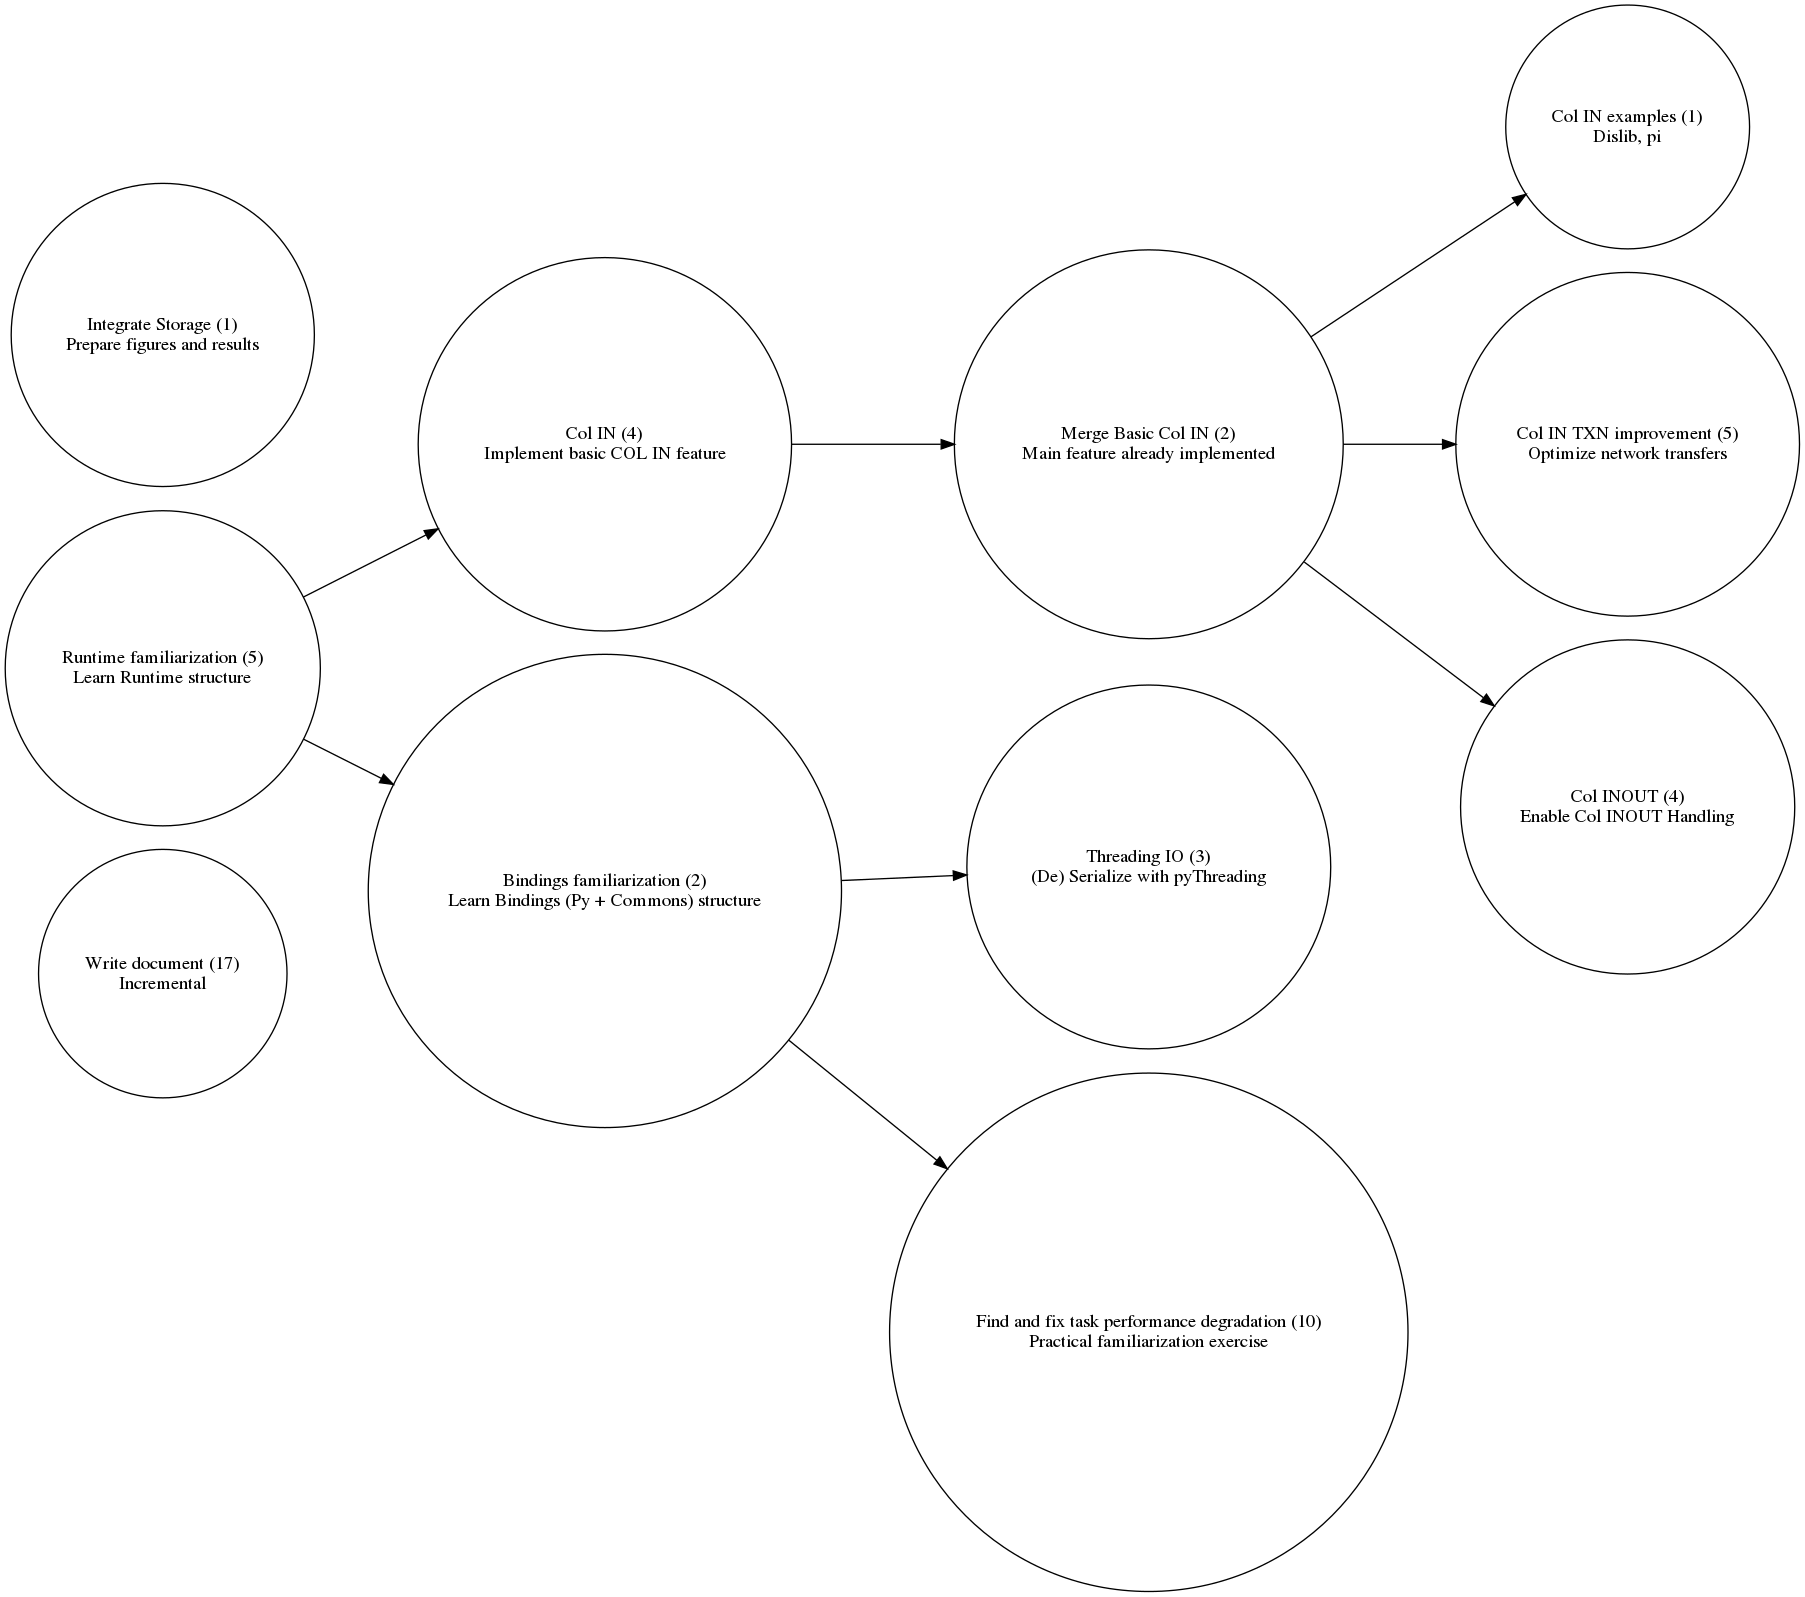
\includegraphics[scale = 0.20]{figures/thesis_task_graph.png}
\label{fig:thesis_task_graph}
\caption{A dependency graph representation of the different tasks and the dependencies between them. The numbers between parentheses denote the estimated number of needed weeks to do some task}
\end{figure}

A more precise explanation of these tasks (and shortcuts to the corresponding sections) can be found below. It is recommended to read the following sections in order to fully understand all the terms and explanations that will appear in this document.

\begin{itemize}
\item \textbf{Runtime familiarization} Some features require a deep knowledge of the COMPSs Runtime. COMPSs is written in Java, so this task will mainly consist of learning the class hierarchy and modules of the Runtime, how to build and deploy it, and how to fix and add features to it. This task is explained and developed mainly in section \ref{subsec:runtime_structure}.

\item \textbf{Bindings familiarization} COMPSs has two bindings that allow the user to write applications for both C/C++ and Python. We will mainly focus on the Python (PyCOMPSs) part. This task will consist of learning the different Python modules, how user code is decorated from there, and how this binding communicates with the COMPSs Runtime via C++ Python extensions \footnote{https://docs.python.org/3/extending/building.html} and the JNI library \footnote{https://es.wikipedia.org/wiki/Java\_Native\_Interface}. The development of this task can be found in section \ref{subsec:pycompss_structure}.

\item \textbf{Collection IN} This feature will allow the user to deal with multiple COMPSs parameters at once if he puts them in some container. This task and all the others that have something to do with it is developed and explained in section \ref{sec:col}.

\item \textbf{Merge Collection IN} This task consists of integrating the changes made in COMPSs to support collections into the main branch of the software while guaranteeing that this integration does not affect the stability and performance of the software. This section includes to implement some kind of unit test, and to include it in a continuous integration environment. COMPSs has many concurrent developers attacking many sections of the software at the same time, and the software has many lines of source code, so this task may no be as trivial as it seems.

\item \textbf{Collection INOUT} Same as collection IN, but allowing inout objects as the content of a collection. The development of this feature can be found in section \ref{subsec:col_inout}.

\item \textbf{Collection Examples} Improve some existing applications with the COLLECTION feature. These examples can be found in section \ref{subsec:col_examples}.

\item \textbf{Collection TXN improvement} The fact that two objects belong to the same collection can be used to our advantage to implement some improvements in how this data is transferred to the destination node. For example, they could be transferred together and then split in the destination. This idea may result in better performance (less simultaneous connections, less bandwith bottleneck) or may make things worse (less parallelism when transferring data between nodes). This last section must be considered as an extra, as the difficulty and the required time to implement it is probably out of the scope and resources of this project, and it is more than likely that it will remain as a possible future work line.

\item \textbf{Combine Storage with PyCOMPSs} One of our approaches towards the improvement of object management is to partially delegate it to some \textit{dedicated} storage backend. This includes the development of some PyCOMPSs API that allows the user to use this backend and to integrate it to the \textit{intelligence} of the COMPSs Runtime. All the work related with this task can be found in section \ref{sec:storage}.

\item \textbf{Threading IO in PyCOMPSs} Most Python implementations have a Global Interpreter Lock (GIL) that prevent parallelism with Python threads. This does not mean that some speedup can be obtained if IO operations are done with Python threads, and that Python programs are necessary sequential or, at best, concurrent (for example, the Numpy library has many linear algebra operations implemented with OpenMP). This task explores if it is worthy to parallelize IO operations with Python threads.

\item \textbf{Find and fix task performance degradation} This task is just a practical exercise aimed to check if we have actually achieved a good enough understanding of the COMPSs programming model. It consists of dealing with a performance decay in a user's application. By dealing we mean to identify the problem, its sources, think about a solution and implement it (if applies). This task is developed in section \ref{sec:task_overhead}. This task is intended to serve as an extension of the explanation on how COMPSs works.

\end{itemize}

\section{Methodology}
This project will be developed in a constant-feedback, results-driven model. That is, the outcome of some implementation may make our initial planning change, as these implementations may reveal more interesting lines, or heavy limitations to the current ones.\\
\\
One of the key aspects of this kind of work is to keep results reachable and easy to reproduce. For this purpose all the contents regarding to this project can be found in two git repositories:
\begin{itemize}
\item \verb|https://github.com/srgrr/TFM| The repository with this document, and all the applications, code snippets and figures contained in it
\item \verb|https://github.com/bsc-wdc/compss| The public mirror of the COMPSs programming model. All executions and applications will contain a reference to the exact commit or tag we used
\end{itemize}
This methodology allows our reviewers to easily reproduce all the experiments and to refer to some pieces of source code mentioned here.\\
\\
All tasks are tracked and annotated in a Trello board. Trello \footnote{https://trello.com/} is an online platform that emulates the classical board with post-its on it. A screenshot depicting the Trello board can be found in figure \ref{fig:trello}.

\begin{figure}
\centering
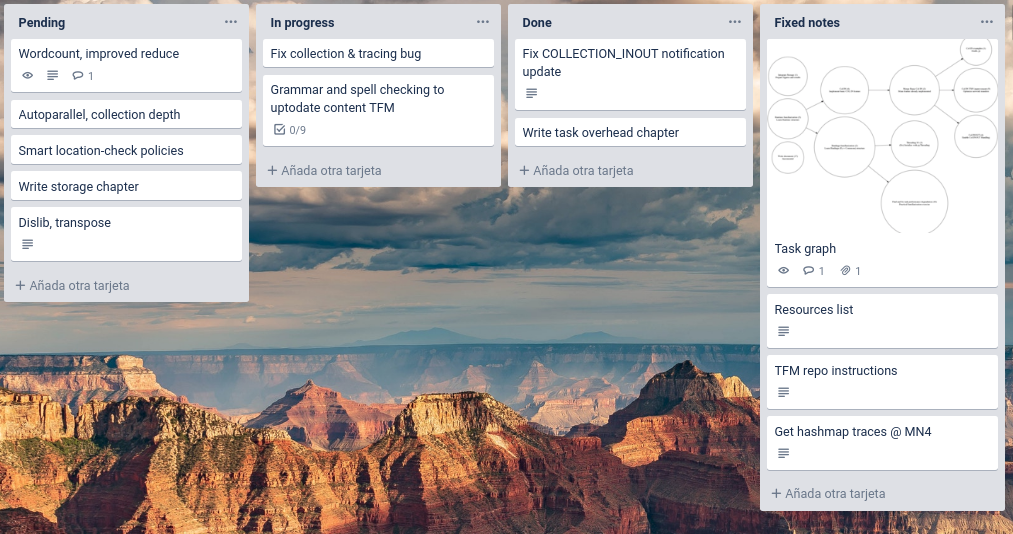
\includegraphics[scale = 0.5]{figures/trello.png}
\caption{A screenshot of the Trello board. Tasks are divided in Pending (tasks we want to do but we are not currently doing), In Progress (tasks we want to do and we are currently doing), and Done (tasks we already did but we want to comment them with our supervisors or other members of our team). We also have some fixed notes with links to useful resources, rules of the project, the task graph, and so on}
\label{fig:trello}
\end{figure}